\section{Code structure}

\castro\ is built upon the \boxlib\ \cpp\ framework.  This provides
high-level classes for managing an adaptive mesh refinement
simulation, including the core data structures we will deal with.  A
key design pattern in \boxlib\ is that the overall memory management
and parallelization is done in the \cpp\ layer, while the heavy
computational work is done in Fortran kernels.  \boxlib\ provides
convenient data structures that allow for this workflow---high level
objects in \cpp\ that communicate with Fortran through pointers to
data regions that appear as multidimensional arrays.

\castro\ uses a structured-grid approach to hydrodynamics.  We work
with square/cubic zones that hold state variables (density, momentum,
etc.)  and compute the fluxes of these quantities through the
interfaces of the zones (this is a finite-volume approach).
Parallelization is achieved by domain decomposition.  We divide our
domain into many smaller boxes, and distributed these across
processors.  When information is needed at the boundaries of the
boxes, messages are exchanged and this data is held in a perimeter of
{\em ghost cells}.  \boxlib\ manages this decompostion and
communication for us.  Additionally, \boxlib\ implements adaptive mesh
refinement.  In addition to the coarse decomposition of our domain
into zones and boxes, we can refine rectangular regions by adding
finer-gridded boxes on top of the coarser grid.  We call the
collection of boxes at the same resolution a {\em level}.

\castro\ uses a hybrid MPI + OpenMP approach to parallelism.  MPI is
at used to communicate across nodes on a computer and OpenMP is used
within a node, to loop over subregions of a box with different
threads.

The code structure in the {\tt Castro/} directory reflects the
division between \cpp\ and Fortran.
\begin{itemize}
\item {\tt constants/}: contains a file of useful constants in CGS units

\item {\tt Docs/}: you're reading this now!

\item {\tt Exec/}: various problem implementations, sorted by category:
  \begin{itemize}
  \item {\tt gravity\_tests/}: test problems that primarily exercise the gravity solver
  \item {\tt hydro\_tests/}: test problems of the hydrodynamics (with or without reactions)
  \item {\tt radiation\_tests/}: test problems that primarily exercise the radiation hydrodynamics solver
  \item {\tt science/}: problem setups that were used for scientific investigations
  \item {\tt unit\_tests/}: test problems that exercise primarily a single module
  \end{itemize}

\item {\tt Microphysics/}: contains directories for different default
  microphysics (these are all implemented in Fortran)
  \begin{itemize}
  \item {\tt conductivity/}: the thermal conductivity
  \item {\tt EOS/}: the equation of state
  \item {\tt networks/}: the nuclear reaction networks
  \end{itemize}

\item {\tt Source/}: source code.  In this main directory is all of
  the \cpp\ code.  The associated Fortran code is in the following
  sub-directories:
  \begin{itemize}
  \item {\tt Src\_1d}: one-dimensional Fortran code
  \item {\tt Src\_2d}: two-dimensional Fortran code
  \item {\tt Src\_3d}: three-dimensional Fortran code
  \item {\tt Src\_nd}: dimension agnostic Fortran code---this is code that
    is written in a generic fashion so that it can be called regardless
    of the dimensionality of the problem.
  \end{itemize}
\item {\tt Util/}: a catch-all for additional things you may need
  \begin{itemize}
  \item {\tt ConvertCheckpoint/}: a tool to convert a checkpoint file to
     a larger domain
  \item $\ldots$
  \end{itemize}


\end{itemize}


\section{Major data structures}

The following data structures are the most commonly encountered when
working in the \cpp\ portions of \castro.  This are all
\boxlib\ data-structures / classes.

\subsection{{\tt Amr}}

This is the main class that drives the whole simulation.  This is
the highest level in \castro.


\subsection{\amrlevel\ and {\tt Castro} classes}

An \code{\amrlevel} is a virtual base class provided by \boxlib\ that
stores all the state data on a single level in the AMR hierarchy and
understands how to advance that data in time.

The most important data managed by the \amrlevel\ is an array of
\statedata, which holds the fluid quantities, etc., in the boxes
that together make up the level.

The {\tt Castro} class is derived from the \amrlevel.  It provides
the \castro-specific routines to evolve our system of equations.  Like
the \amrlevel, there is one {\tt Castro} object for each level in the
AMR hierarchry.

A lot of the member data in the {\tt Castro} class are static member
variables---this means that they are shared across all instances of
the class.  So, in this case, every level will have the same data.
This is done, in particular, for the values of the runtime parameters,
but also for the {\tt Gravity}, {\tt Diffusion}, and {\tt Radiation}
objects.  This means that those objects cover all levels and are the
same object in each instantiation of the {\tt Castro} class.

\subsection{Floating point data}

Floating point data in the \cpp\ \boxlib\ frame work is declared as
{\tt Real}.  This is {\tt typedef} to either {\tt float} or {\tt
  double} depending on the make variable \makevar{PRECISION}.

At present, single precision is not supported in \castro.  This is
because the Fortran routines that we interact with are all written to
accept double precision inputs.

\subsection{\bbox\ and \farraybox}

A \code{\bbox} is simply a rectangular region in space.  It does not hold
data.  In \boxlib, an AMR level has a global index space, with
$(0,0,0)$ being the lower left corner of the domain at that level, and
$(N_x-1, N_y-1, N_z-1)$ being the upper right corner of the domain
(for a domain of $N_x \times N_y \times N_z$ zones).  The location of
any \bbox\ at a level can be uniquely specified with respect to this
global index space by giving the index of its lower-left and
upper-right corners.  Figure~\ref{fig:soft:indexspace} shows an
example of three boxes at the same level of refinement.

\boxlib\ provides other data structures that collect \bbox es together,
most importantly the \code{\boxarray}.  We generally do not use these
directly, with the exception of the \boxarray\ \variable{grids},
which is defined as part of the \amrlevel\ class that {\tt Castro}
inherits. {\tt grids} is used when building new \multifab s to give
the layout of the boxes at the current level.

\begin{figure}[t]
\centering
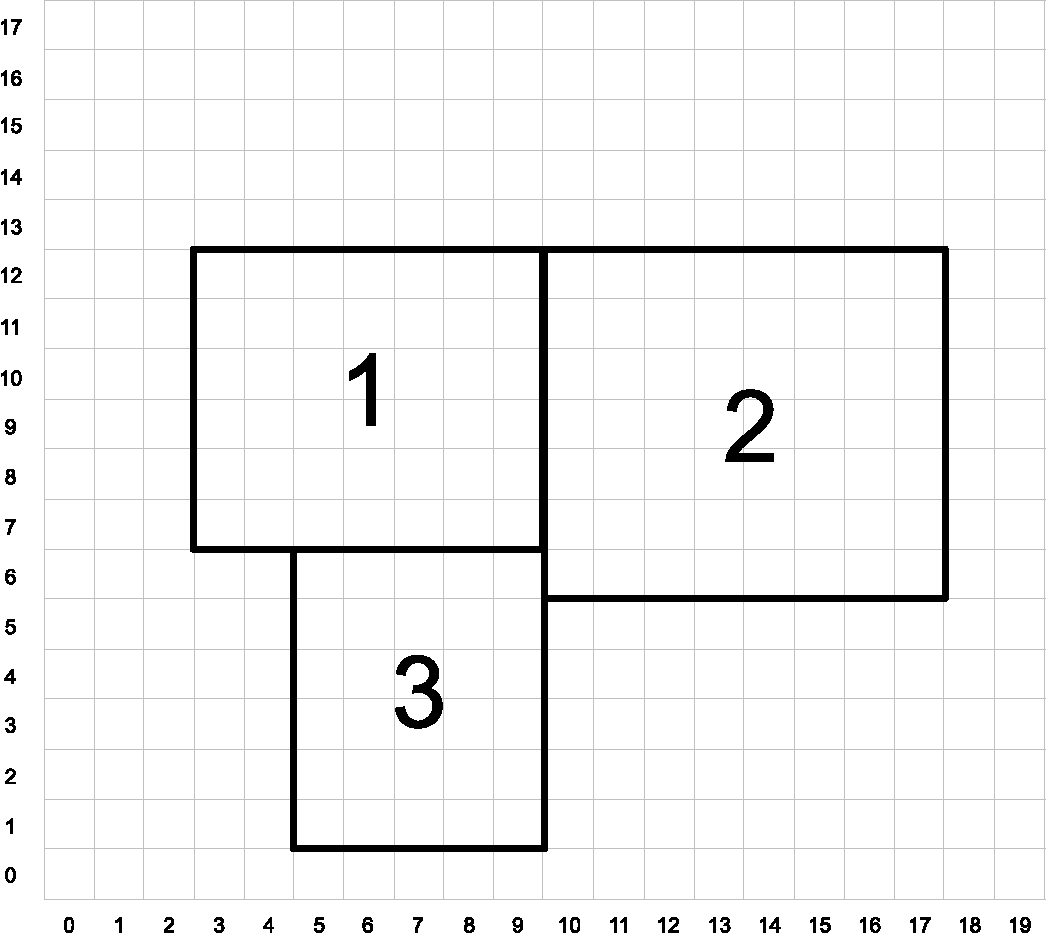
\includegraphics[width=4.0in]{index_grid2}
\caption[Single-level grid structure]
{\label{fig:soft:indexspace} Three boxes that comprise a single level.  At this
  resolution, the domain is 20$\times$18 zones.  Note that the
  indexing in BoxLib starts with $0$.}
\end{figure}


A \code{\farraybox} or {\em FAB}, for {\em Fortran array box} is a data
structure that contains a \bbox\ locating it in space, as well as a
pointer to a data buffer.  The real floating point data are stored as
one-dimensional arrays in \farraybox es.  The associated \bbox can be
used to reshape the 1D array into multi-dimensional arrays to be used
by Fortran subroutines.  The key part of the \cpp\ \boxlib\ data
structures is that this data buffer can be sent to Fortran, where it
will appear as a {\tt DIM}+1 dimensional array ({\tt DIM} space + 1
component).

Note: \castro\ is complied for a specific dimensionality.


\subsection{\multifab}

At the highest abstraction level, we have the \code{\multifab} (mulitple
\farraybox es).  A \multifab\ contains an array of \bbox es, including
\bbox es owned by other processors for the purpose of communication,
an array of MPI ranks specifying which MPI processor owns each \bbox,
and an array of pointers to \farraybox es owned by this MPI
processor. \MarginPar{is this still an accurate description?}  Note: a
\multifab\ is a collection of the boxes that together make up a single
level of data in the AMR hierarchy.

A \multifab\ can have multiple components (like density, temperature,
...) as well as a perimeter of ghost cells to exchange data with
neighbors or implement boundary conditions (this is all reflected in
the underlying \farraybox).

Parallelization in \boxlib\ is done by distributing the FABs across
processors.  Each processor knows which FABs are local to it.  To loop
over all the boxes local to a processor, an \mfiter\ is used (more
on this below).

High-level operations exist on \multifab s to add, subtract, multiply,
etc., them together or with scalars, so you don't need to write out
loops over the data directly.

In \castro, \multifab s are one of the main data structures you will
interact with in the \cpp\ portions of the code.


\subsection{\statedata}

\code{\statedata} is a class that essentially holds a pair of \multifab s: one
at the old time and one at the new time.  \boxlib\ knows how to
interpolate in time between these states to get data at any
intermediate point in time.  The main data that we care about in
\castro\ (the fluid state, gravitational potential, etc.) will be
stored as \statedata.  Essentially, data is made \statedata\ in
\castro\ if we need it to be stored in checkpoints / plotfiles, and/or
we want it to be automatically interpolated when we refine.

An \amrlevel\ stores an array of \statedata\ (in a \cpp\ array
called {\tt state}).  We index this array using integer keys (defined
via an {\tt enum} in {\tt Castro.H}).  The state data is registered
with \boxlib\ in \code{Castro\_setup.cpp}.

Note that each of the different \statedata\ carried in the {\tt state}
array can have different numbers of components, ghost cells, boundary
conditions, etc.  This is the main reason we separate all this data
into separate \statedata\ objects collected together in an indexable
array.

The current \statedata\ names  \castro\ carries are:
\begin{itemize}
\item \variable{State\_Type} : this is the {\tt NUM\_STATE} hydrodynamics
  components that make up the conserved hydrodynamics state (usually
  referred to as $\Ub$ in these notes.  But note that this does
  not include the radiation energy density.

  In Fortran, the components of a FAB derived from {\tt State\_Type}
  is indexed using the integer keys defined in \code{Castro\_nd.F90}
  and stored in \code{meth\_params\_module}, e.g., {\tt URHO}, {\tt UMX},
  {\tt UMY}, ...

  Note: regardless of dimensionality, we always carry around all
  three velocity components.  The ``out-of-plane'' components
  will simply be advected, but we will allow rotation (in particular,
  the Coriolis force) to affect them.

  {\tt State\_Type} \multifab s have no ghost cells by default
  (although, there is an option to force them to have ghost cells by
  setting the parameter \runparam{castro.state\_nghost} at runtime).

  Note that the prediction of the hydrodynamic state to the interface
  will require 4 ghost cells.  This accomodated by creating a separate
  \multifab, \variable{Sborder} that lives at the old-time level and
  has the necessary ghost cells.  We will describe this more later.

\item \variable{Rad\_Type} : this stores the radiation energy density,
  commonly denoted $E_r$ in these notes.  It has \variable{nGroups}
  components---the number of energy groups used in the multigroup
  radiation hydrodynamics approximation. \MarginPar{not sure how
    neutrinos factor in here}

\item \variable{PhiGrav\_Type} : this is simply the gravitational
  potential, usually denoted $\Phi$ in these notes.

\item \variable{Gravity\_Type} : this is the gravitational
  acceleration. There are always 3 components, regardless of the
  dimensionality (consistent with our choice of always carrying all 3
  velocity components).

\item \variable{PhiRot\_Type} : this is the rotational potential.
  When rotation is enabled, this will store the effective potential
  corresponding to the centrifugal force. 

\item \variable{Rotation\_Type} : this is the rotational acceleration.
  There are always 3 components, regardless of the dimensionality
  (consistent with our choice of always carrying all 3 velocity
  components).  This includes the terms corresponding to the Coriolis
  force, the centrifugal force, as well as optional terms due to the
  change in rotation rate, $\Omega$.

\item \variable{Source\_Type} : this holds the time-rate of change of
  the source terms, $d\Sb/dt$, for each of the {\tt NUM\_STATE} {\tt
    State\_Type} variables.

  Note: we do not make use of the old-time quantity here. In fact, we
  never allocate the \farraybox s for the old-time in the {\tt Source\_Type}
  \statedata, so there is not wasted memory.

\item \variable{Reactions\_Type} : this holds the data for the nuclear
  reactions.  It has {\tt NumSpec+2} components: the species
  creation rates (usually denoted $\omegadot_k$ in these notes),
  the specific energy generation rate ($\dot{e}_\mathrm{nuc}$),
  and its density ($\rho \dot{e}_\mathrm{nuc}$).  

  These are stored as \statedata\ so we have access to the reaction terms
  outside of advance, both for diagnostics (like flame speed estimation)
  and for reaction timestep limiting (this in particular needs the 
  data stored in checkpoints for continuity of timestepping upon restart).

\MarginPar{why do we need rho edot and edot separately?}

\item \variable{SDC\_Source\_Type} : this is used with the SDC
  time-advancement algorithm (not the default Strang-splitting
  algorithn).  This will store the {\tt NUM\_STATE} advective source
  terms for use in the evolution of the reactive terms in the SDC
  advancement.

\item \variable{SDC\_React\_Type} : this is used with the SDC
  time-advancement algorithm.  This stores the {\tt QVAR} terms
  that describe how the primitive variables change over the timestep
  due only to reactions.  These are used when predicting the interface
  states of the primitive variables for the hydrodynamics portion of the
  algorithm.

\end{itemize}

We access the multifabs that carry the data of interest by interacting
with the \statedata\ using one of these keys.  For instance:
\begin{lstlisting}
MultiFab& S_new = get_new_data(State_Type);
\end{lstlisting}
gets a pointer to the multifab containing the hydrodynamics state data
at the new time.



\subsection{\code{\parray}}

The {\tt PArray<T>} class is similar to the \cpp\ {\tt Array<T>} class,
but it manages an array of pointers to objects of type {\tt T}, rather
than the objects themself.  There are additional options that control
whether the objects are deleted or the pointers simply destructed.

In \castro\, this will commonly be used with \multifab s.


\section{\mfiter\ and interacting with Fortran}

The process of looping over boxes at a given level of refinement and
operating on their data in Fortran is linked to how \castro\ achieves
thread-level parallelism.  The OpenMP approach in \castro\ has evolved
considerably since the original paper was written, with the modern
approach, called {\em tiling}, gearing up to meet the demands of
many-core processors in the next-generation of supercomputers.  We
discuss the original and new approach together here.

In both cases, the key construct is the \code{\mfiter}---this is a
\cpp\ iterator that knows how to loop over the \farraybox es in the
\multifab\ that are local to the processor (in this way, a lot of the
parallelism is hidden from view).

\subsection{Non-Tiling \mfiter}

The non-tiling way to iterate over the \farraybox s is
\footnote{Note: some older code will use a special \boxlib\ preprocessor macro,
\code{BL\_TO\_FORTRAN}, defined in \code{ArrayLim.H}, that converts
the \cpp\ multifab into a Fortran array and its {\tt lo} and {\tt hi} indices.
Additionally, some older code will wrap the Fortran subroutine name
in an additional preprocessor macro, \code{BL\_FORT\_PROC\_CALL}
to handle the name mangling between Fortran and C.  This later
macro is generally not needed any more because of Fortran 2003
interoperability with C (through the Fortran {\tt bind} keyword).
}:
\begin{lstlisting}[language=C++]
  for (MFIter mfi(mf); mfi.isValid(); ++mfi) // Loop over boxes
  {
    // Get the index space of this iteration
    const Box& box = mfi.validbox();

    // Get a reference to the FAB, which contains data and box
    FArrayBox& fab = mf[mfi];

    // Get the index space for the data region in th FAB.
    // Note "abox" may have ghost cells, and is thus larger than
    // or equal to "box" obtained using mfi.validbox().
    const Box& abox = fab.box();

    // We can now pass the information to a Fortran routine,
    // fab.dataPtr() gives a double*, which is reshaped into
    // a multi-dimensional array with dimensions specified by
    // the information in "abox". We will also pass "box",
    // which specifies our "work" region.
    do_work(ARLIM_3D(box.loVect()), ARLIM_3D(box.hiVect()),
            fab.dataPtr(), fab.nComp(),
            ARLIM_3D(abox.loVect()), ARLIM_3D(abox.hiVect())

  }
\end{lstlisting}
A few comments about this code
\begin{itemize}
\item In this example, we are working off of a \multifab\ named {\tt mf}.
  This could, for example, come from state data as:
\begin{lstlisting}
 MultiFab& mf = get_old_data(State_Type);
\end{lstlisting}

\item We are passing the data in {\tt mf} one box at a time to the
  Fortran function {\tt do\_work}.

\item Here the \mfiter\ iterator, {\tt mfi}, will perform the loop
  only over the boxes that are local to the MPI task.  If there are 3
  boxes on the processor, then this loop has 3 iterations.

  {\tt ++mfi} iterates to the next \farraybox\ owned by the
  \multifab\ {\tt mf}, and {\tt mfi.isValid()} returns {\tt false}
  after we've reached the last box contained in the MultiFab,
  terminating the loop.

\item {\tt box} as returned from {\tt mfi.validbox()} does not include
   ghost cells.  This is the valid data region only.
   We can get the indices of the valid zones as {\tt box.loVect()} and
   {\tt box.hiVect()}.

   In passing to the Fortran function, we use the macro
   \code{ARLIM\_3D}, defined in \code{ArrayLim.H} to pass the {\tt lo}
   and {\tt hi} vectors as pointers to an {\tt int} array.  This array
   is defined to always be 3D, with {\tt 0}s substituted for the
   higher dimension values if we are running in 1- or 2D.

   Passing the data in this 3D fashion is a newer approach in \castro.
   This enables writing {\em dimension agnostic code}, like that found
   in {\tt Src\_nd/}.  There are many other approaches that will pass
   only the {\tt DIM} values of {\tt lo} and {\tt hi} using alternate
   macros in {\tt ArrayLim.H}.

\item {\tt fab.dataPtr()} returns a {\tt double *}---a pointer to the
  data region.  This is what is passed to Fortran.

\item {\tt fab.nComp()} gives an {\tt int}---the number of components
  in the \multifab.  This will be used for dimensioning in Fortran.

\item To properly dimension the array in Fortran, we need the actual
  bounds of the data region, including any ghost cells.  This is the
  \bbox\ {\tt abox}, obtained as {\tt fab.box()}.  We pass the {\tt
    lo} and {\tt hi} of the full data region as well.

\end{itemize}

To properly compile, we need a prototype for the Fortran
function.  These are placed in the {\tt *\_F.H} files in the
\castro\ {\tt Source/} directory.  Here's the prototype for
our function:

\begin{lstlisting}[language=C++]
  void do_work
    (const int* lo, const int* hi,
     Real* state, const Real& ncomp
     const int* s_lo, const int* s_hi)
\end{lstlisting}

A few comments on the prototype:
\begin{itemize}
\item we use the {\tt const} qualifier on the many of the arguments.
  This indicates that the data that is pointed to cannot be
  modified\footnote{the way to read these complicated
    \cpp\ declarations is right-to-left.  So `const int* lo` means
    `lo` is a integer pointer to a memory space that is constant.  See
    \url{https://isocpp.org/wiki/faq/const-correctness\#ptr-to-const}}
    means that the pointers themselves are to be unmodified.  But the
    contents of the memory space that they point to can be modified.

\item For {\tt ncomp}, we in the calling sequence, we just did {\tt
  fab.nComp()}.  This returns a {\tt int}.  But Fortran is a
  pass-by-reference language, so we make the argument in the prototype
  a reference.  This ensures that it is passed by reference.
\end{itemize}

In our Fortran example, we want to loop over all of the data,
including 1 ghost cell all around.  The corresponding Fortran function
will look like:
\begin{lstlisting}[language=Fortran]
  subroutine do_work(lo, hi, &
                     state, ncomp, &
                     s_lo, s_hi) bind(C, name="do_work")

    use prob_params_module, only : dg

    integer, intent(in) :: lo(3), hi(3)
    integer, intent(in) :: s_lo(3), s_hi(3), ncomp

    real (kind=dp_t), intent(inout) :: state(s_lo(1):s_hi(1), &
                                             s_lo(2):s_hi(2), &
                                             s_lo(3):s_hi(3), ncomp)

    ! loop over the data
    do k = lo(3)-1*dg(3), hi(3)+1*dg(3)
       do j = lo(2)-1*dg(2), hi(2)+1*dg(2)
          do i = lo(1)-1*dg(1), hi(1)+1*dg(1)

             ! work on state(i,j,k,:), where the last index
             ! is the component of the multifab

          enddo
       enddo
    enddo

  end subroutine do_work
\end{lstlisting}

Finally, comments on the Fortran routine;
\begin{itemize}
\item We use the Fortran 2003 {\tt bind} keyword to specify
  that we want this to be interoperable with C.  Ordinarily
  we would not need to specify the optional argument {\tt name}
  in the binding, but the PGI compiler requires this if our
  Fortran subroutine is part of a module.

\item We dimension state using {\tt s\_lo} and {\tt s\_hi}---these are
  the bounds we got from the \farraybox, and are for the entire data
  region, including ghost cells.

  Note, in Fortran, the spatial indices of {\tt state} don't
  necessarily start at {\tt 1}---they reflect the global index space
  for the entire domain at this level of refinement.  This means that
  we know where the box is located.

  Later we'll see how to compute the spatial coordinates using this
  information.

\item Our loop uses {\tt lo} and {\tt hi}---these are the indices
  of the valid data region (no ghost cells).  Since we want a single
  ghost cell all around, we subtract {\tt 1} from {\tt lo} and add {\tt 1}
  to {\tt hi}.

  Finally, since this is dimension-agnostic code (it should work
  correctly in 1-, 2-, and 3D), we need to ensure the loops over the
  higher dimensions do nothing when we compile for a lower
  dimensionality.  This is the role of {\tt dg}---{\tt dg} is {\tt 1}
  if our simulation includes that spatial dimension and {\tt 0}
  otherwise.

  If we were not looping over ghost cells too, then we would not need
  to invoke {\tt dg}, since {\tt lo} and {\tt hi} are both set to {\tt
    0} for any dimensions not represented in our simulation.

\end{itemize}

Up to this point, we have not said anything about threading.  In this
style of using the \mfiter, we implement the OpenMP in Fortran, for
instance by putting a pragma around the outer loop in this example.


\subsection{\boxlib's Current Tiling Approach In C++}
\label{sec:boxlib1}

There are two types of tiling that people discuss.  In {\em logical
tiling}, the data storage in memory is unchanged from how we do things
now in pure MPI.  In a given box, the data region is stored
contiguously).  But when we loop in OpenMP over a box, the tiling
changes how we loop over the data.  The alternative is called {\em
separate tiling}---here the data storage in memory itself is changed
to reflect how the tiling will be performed.  This is not considered
in \boxlib.

We have recently introduced logical tiling into parts of \boxlib\.  It
is off by default, to make the transition smooth and because not
everything should be tiled.  It can be enabled on a loop-by-loop basis
by setting an optional argument to \mfiter.  We demonstrate this
below.  Further examples can be found at {\tt Tutorials/Tiling\_C},
and {\tt Src/LinearSolvers/C\_CellMG/}.

In our logical tiling approach, a box is logically split into tiles,
and a {\tt MFIter} loops over each tile in each box.  Note that the
non-tiling iteration approach can be considered as a special case of
tiling with the tile size equal to the box size.

Let us consider an example.  Suppose there are four boxes---see
Figure~\ref{fig:domain-tiling}.
\begin{figure}[t]
\centering
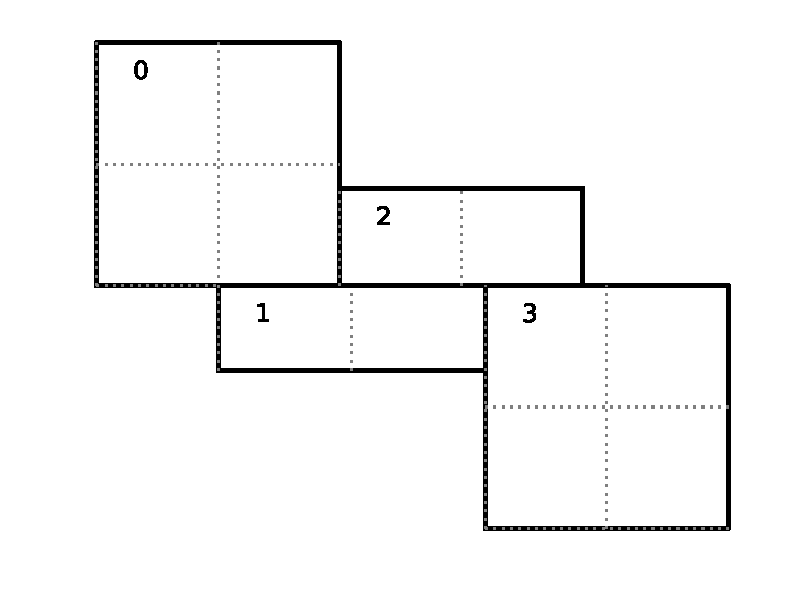
\includegraphics[width=0.8\linewidth]{domain-tile}
\caption{\label{fig:domain-tiling} A simple domain showing 4
  {\tt Box}es labeled 0--3, and their tiling regions (dotted lines)}
\end{figure}
%
The first box is divided into 4 logical tiles, the second and third
are divided into 2 tiles each (because they are small), and the fourth
into 4 tiles.  So there are 12 tiles in total.  The difference between
the tiling and non-tiling version are then:

\begin{itemize}
\item In the tiling version, the loop body will be run 12 times.  Note
  that {\tt tilebox} is different for each tile, whereas {\tt fab}
  might be referencing the same object if the tiles belong to the same
  box.

\item In the non-tiling version (by constructing {\tt MFIter} without
  the optional second argument or setting to {\tt false}), the loop
  body will be run 4 times because there are four boxes, and a call to
  {\tt mfi.tilebox()} will return the traditional {\tt validbox}.  The
  non-tiling case is essentially having one tile per box.
\end{itemize}


The tiling implementation of the same call to our the Fortran {\tt
  do\_work} routine is show below:

\begin{lstlisting}[language=C++]
  bool tiling = true;
  for (MFIter mfi(mf, tiling); mfi.isValid(); ++mfi) // Loop over tiles
  {
    // Get the index space of this iteration.
    const Box& box = mfi.growntilebox(1);

    // Get a reference to the FAB, which contains data and box
    FArrayBox& fab = mf[mfi];

    // Get the index space for the data pointed by the double*.
    const Box& abox = fab.box();

    // We can now pass the information to a Fortran routine.
    do_work(ARLIM_3D(box.loVect()), ARLIM_3D(box.hiVect()),
            fab.dataPtr(), fab.nComp(),
            ARLIM_3D(abox.loVect()), ARLIM_3D(abox.hiVect())

  }
\end{lstlisting}
Note that the code is almost identical to the one in \S~\ref{sec:boxlib0}.
Some comments:
\begin{itemize}
\item The iterator now takes an extra argument to turn on tiling (set
  to {\tt true}).  

  There is another interface fo {\tt MFIter} that can take an {\tt
    IntVect} that explicitly gives the tile size in each coordinate
  direction.  If we don't explictly specify the tile size at the loop,
  then the runtime parameter \runparam{fabarray.mfiter\_tile\_size}
  can be used to set it globally.

\item {\tt .validBox()} has the same meaning as in the non-tile
  approach, so we don't use it.  
  Since in this example, we want to include a single ghost cell in our
  loop over the data, we use {\tt .growntilebox(1)} (where the {\tt 1}
  here indicates a single ghost cells) to get the {\tt Box} (and
  corresponding {\tt lo} and {\tt hi}) for the {\em current tile}, not
  the entire data region.  If instead, we just wanted the valid
  region in Fortran, without any ghost cells, we would use {\tt
    .tilebox()}.

\item When passing into the Fortran routine, we still use the index
  space of the entire \farraybox\ (including ghost cells), as seen in
  the {\tt abox} construction.  This is needed to properly dimension
  the array in Fortran.  

  The Fortran routine will declare a multidimensional array that is of
  the same size as the entire box, but only work on the index space
  identified by the tile-box ({\tt box}).
\end{itemize}

The Fortran code is almost the same as before, but now our loop 
simply uses {\tt lo} and {\tt hi}, since, by construction with
{\tt .growntilebox(1)}, this already includes the single ghost cell 
all around:
\begin{lstlisting}[language=Fortran]
  subroutine do_work(lo, hi, &
                     state, ncomp, &
                     s_lo, s_hi) bind(C, name="do_work")

    integer, intent(in) :: lo(3), hi(3)
    integer, intent(in) :: s_lo(3), s_hi(3), ncomp

    real (kind=dp_t), intent(inout) :: state(s_lo(1):s_hi(1), &
                                             s_lo(2):s_hi(2), &
                                             s_lo(3):s_hi(3), ncomp)

    ! loop over the data
    do k = lo(3), hi(3)
       do j = lo(2), hi(2)
          do i = lo(1), hi(1)

             ! work on state(i,j,k,:), where the last index
             ! is the component of the multifab

          enddo
       enddo
    enddo

  end subroutine do_work
\end{lstlisting}

The function prototype is unchanged.

Tiling provides us the opportunity of a coarse-grained approach for
OpenMP.  Threading can be turned on by inserting the following line
above the {\tt for (MFIter...)} line.
\begin{lstlisting}
  #pragma omp parallel
\end{lstlisting}
Note that the OpenMP pragma does not have a {\tt for}---this is not
used when working with an iterator.

Assuming four threads are used in the above example, thread 0 will
work on 3 tiles from the first box, thread 1 on 1 tile from the first
box and 2 tiles from the second box, and so forth.  Note that
OpenMP can be used even when tiling is turned off.  In that case, the
OpenMP granularity is at the box level (and good performance would need
many boxes per MPI task).

The tile size for the three spatial dimensions can be set by a
parameter, e.g., {\tt fabarray.mfiter\_tile\_size = 1024000 8 8}.  A
huge number like {\tt 1024000} will turn off tiling in that direction.
As noted above, the {\tt MFIter} constructor can also take an explicit
tile size: {\tt MFIter(mfi(mf,IntVect(128,16,32)))}.

Note that tiling can naturally transition from all threads working
on a single box to each thread working on a separate box as the boxes
coarsen (e.g., in multigrid).

The {\tt MFIter} class provides some other useful functions:
\begin{itemize}
  \item {\tt mfi.validbox()} : The same meaning as before independent of tiling.

  \item {\tt mfi.tilebox()} : The standard way of getting the bounds of the 
    current tile box.  This will tile over the valid data region only.

  \item {\tt mfi.growntilebox(int)} : A grown tile box that includes
    ghost cells at box boundaries only.  Thus the returned boxes for a
    \farraybox\ are non-overlapping.

  \item {\tt mfi.nodaltilebox(int)} : Returns non-overlapping
    edge-type boxes for tiles.  The argument is for direction.

  \item {\tt mfi.fabbox()}  : Same as mf[mfi].box().
\end{itemize}

Finally we note that tiling is not always desired or better.  The
traditional fine-grained approach coupled with dynamic scheduling is
more appropriate for work with unbalanced loads, such as chemistry
burning in cells by an implicit solver.  Tiling can also create extra
work in the ghost cells of tiles.


\subsubsection{Practical Details in Working with Tiling}

With tiling, the OpenMP is now all in \cpp, and not in Fortran for all
modules except reactions and {\tt initdata}.  

It is the responsibility of the coder to make sure that the routines
within a tiled region are safe to use with OpenMP.  In particular,
note that:
\begin{itemize}
\item tile boxes are non-overlapping
\item the union of tile boxes completely cover the valid region of the
  fab
\item Consider working with a node-centered MultiFab, {\tt ugdnv}, and
  a cell-centered MultiFab, {\tt s}:
  \begin{itemize}

  \item with {\tt mfi(s)}, the tiles are based on the cell-centered
    index space.  If you have an $8\times 8$ box, then and 4 tiles,
    then your tiling boxes will range from $0\rightarrow 3$,
    $4\rightarrow 7$.

  \item with {\tt mfi{ugdnv}}, the tiles are based on nodal indices,
    so your tiling boxes will range from $0\rightarrow 3$,
    $4\rightarrow 8$.

  \end{itemize}

\item When updating routines to work with tiling, we need to
  understand the distinction between the index-space of the entire box
  (which corresponds to the memory layout) and the index-space of the
  tile.

  \begin{itemize}

  \item In the \cpp\ end, we pass (sometimes via the {\tt
    BL\_TO\_FORTRAN()} macro) the {\tt loVect} and {\tt hiVect} of the
    entire box (including ghost cells).  These are then used to
    allocate the array in Fortran as:
\begin{lstlisting}
  double precision :: a(a_l1:a_h1, a_l2:a_h2, ...)
\end{lstlisting}
    When tiling is used, we do not want to loop as {\tt do a\_l1,
      a\_h1}, but instead we need to loop over the tiling region.  The
    indices of the tiling region need to be passed into the Fortran
    routine separately, and they come from the {\tt mfi.tilebox()}
    or {\tt mfi.growntilebox()} statement.

  \item In Fortran, when initializing an array to {\tt 0}, do so only
    over the tile region, not for the entire box.  For a Fortran array
    {\tt a}, this means we cannot do:
\begin{lstlisting}
  a = 0.0
  a(:,:,:,:) = 0.0
\end{lstlisting}
    but instead must do:
\begin{lstlisting}
  a(lo(1):hi(1),lo(2):hi(2),lo(3):hi(3),:) = 0.0
\end{lstlisting}
    where {\tt lo()} and {\tt hi()} are the index-space for the tile box
    returned from {\tt mfi.tilebox()} in \cpp\ and passed into the Fortran
    routine.

\item Look at {\tt r\_old\_s} in {\tt Exec/gravity\_tests/DustCollapse/probdata.f90} as an
  example of how to declare a {\tt threadprivate} variable---this is then used
  in {\tt sponge\_nd.f90}.

\end{itemize}

\end{itemize}



\section{Boundaries: {\tt FillPatch} and {\tt FillPatchIterator}}

\boxlib\ calls the act of filling ghost cells a {\em fillpatch}
operation.  Boundaries between grids are of two types. The first we
call ``fine-fine'', which is two grids at the same level.  The second
type is "coarse-fine", which needs interpolation from the coarse grid
to fill the fine grid ghost cells.  Both of these are part of the
fillpatch operation.  Fine-fine fills are just a straight copy from
``valid regions'' to ghost cells.  Coarse-fine fills are enabled
because the \statedata\ is not just arrays, they're ``State Data'',
which means that the data knows how to interpolate itself (in an
anthropomorphical sense).  The type of interpolation to use is defined
in {\tt Castro\_setup.cpp}---search for {\tt
  cell\_cons\_interp}, for example---that's ``cell conservative
interpolation'', i.e., the data is cell-based (as opposed to
node-based or edge-based) and the interpolation is such that the
average of the fine values created is equal to the coarse value from
which they came.  (This wouldn't be the case with straight linear
interpolation, for example.)

Additionally, since \statedata\ has an old and new timelevel, 
the fill patch operation can interpolate to an intermediate time.

\subsection{Examples}

To illustrate the various ways we fill ghost cells and use the data,
let's consider the following scenarios:


\begin{itemize}

\item {\em You have state data that was defined with no ghost cells.  You
  want to create a new \multifab\ containing a copy of that data with
  {\tt NGROW} ghost cells.}

  This is the case with \variable{Sborder}---the \multifab\ of the
  hydrodynamic state that we use to kick-off the hydrodynamics 
  advance.

  {\tt Sborder} is declared in {\tt Castro.H} simply as:
\begin{lstlisting}[language=C++]
  Multifab Sborder;
\end{lstlisting}

  It is then allocated in \code{Castro::initialize\_do\_advance()}
\begin{lstlisting}[language=C++]
  Sborder.define(grids, NUM_STATE, NUM_GROW, Fab_allocate);                   
  const Real prev_time = state[State_Type].prevTime();                        
  expand_state(Sborder, prev_time, NUM_GROW);      
\end{lstlisting}
  Note in the call to {\tt .define()}, we tell \boxlib\ to already
  allocate the data regions for the \farraybox s that are part of {\tt
    Sborder}.

  The actually filling of the ghost cells is done by
  \code{Castro::expand\_state()}:
\begin{lstlisting}[language=C++]
  AmrLevel::FillPatch(*this, Sborder, NUM_GROW, 
                      prev_time, State_Type, 0, NUM_STATE);                
\end{lstlisting}
  Here, we are filling the {\tt ng} ghost cells of \multifab {\tt
    Sborder} at time {\tt prev\_time}.  We are using the
  \statedata\ that is part of the current {\tt Castro} object that we
  are part of.  Note: {\tt FillPatch} takes an object reference as its
  first argument, which is the object that contains the relevant
  \statedata---that is what the {\tt *this} pointer indicates.
  Finally, we are copying the {\tt State\_Type} data components 0 to
  {\tt NUM\_STATE}\footnote{for clarity and continuity in this
    documentation, some of the variable names have been changed
    compared to the actual code}.

The result of this operation is that {\tt Sborder} will now have
{\tt NUM\_GROW} ghost cells consistent with the {\tt State\_Type}
data at the old time-level.

\item {\em You have state data that was defined with {\tt NGROW} ghost
  cells.  You want to ensure that the ghost cells are filled
  (including any physical boundaries) with valid data.}

  This is very similar to the procedure shown above.  The main
  difference is that for the \multifab\ that will be the target
  of the ghost cell filling, we pass in a reference to the \statedata\
  itself.  

  The main thing you need to be careful of here, is that you 
  need to ensure that the the time you are at is consistent with
  the \statedata's time.  Here's an example from the radiation
  portion of the code {\tt MGFLDRadSolver.cpp}:

\begin{lstlisting}[language=C++]
  Real time = castro->get_state_data(Rad_Type).curTime();
  MultiFab& S_new = castro->get_new_data(State_Type);

  AmrLevel::FillPatch(*castro, S_new, ngrow, time, State_Type,
                      0, S_new.nComp(), 0); 
\end{lstlisting}

  In this example, {\tt S\_new} is a pointer to the new-time-level
  {\tt State\_Type} \multifab.  So this operation will use the {\tt
    State\_Type} data to fill its own ghost cells.  we fill the {\tt
    ngrow} ghost cells of the new-time-level {\tt State\_Type} data,
  for all the components.

  Note that in this example, because the \statedata\ lives in the {\tt
    Castro} object and we are working from the {\tt Radiation} object,
  we need to make reference to the current {\tt castro} object
  pointer.  If this were all done within the {\tt Castro} object, then
  the pointer will simply be {\tt *this}, as we saw above.

\item {\em You have a \multifab\ with some derived quantity.  You want to
  fill its ghost cells.}

  \multifab s have a {\tt FillBoundary()} method that will fill all
  the ghost cells between boxes at the same level.  It will not fill
  ghost cells at coarse-fine boundaries or at physical boundaries.  \MarginPar{what is the use case for this?}

\item {\em You want to loop over the FABs in state data, filling ghost cells
  along the way}

  This is the job of the \code{\fillpatchiterator}---this iterator is used to
  loop over the grids and fill ghostcells.  A key thing to keep in
  mind about the \fillpatchiterator\ is that you operate on a copy
  of the data---the data is disconnected from the original source.  If
  you want to update the data in the source, you need to explicitly
  copy it back.  Also note: {\tt FillPatchIterator} takes a multifab,
  but this is not filled---this is only used to get the grid
  layout.  Finally, the way the \fillpatchiterator\ is implemented
  is that all the communication is done first, and then the iterating
  over boxes commences.

  For example, the loop that calls {\tt CA\_UMDRV} (all the
  hydrodynamics integration stuff) starts with
\begin{lstlisting}
   for (FillPatchIterator fpi(*this, S_new, NUM_GROW,
                              time, State_Type, strtComp, NUM_STATE);
         fpi.isValid(); ++fpi)
   {
     FArrayBox &state = fpi();
     Box bx(fpi.validbox());

     // work on the state FAB.  The interior (valid) cells will 
     // live between bx.loVect() and bx.hiVect()
   }
\end{lstlisting}
Here the {\tt FillPatchIterator} is the thing that distributes the
grids over processors and makes parallel ``just work''. This fills the
single patch ``{\tt fpi}'' , which has {\tt NUM\_GROW} ghost cells,
with data of type ``{\tt State\_Type}'' at time ``{\tt time}'',
starting with component {\tt strtComp} and including a total of {\tt
  NUM\_STATE} components. \MarginPar{how do tiling and \fillpatchiterator\ work together?}

\end{itemize}

In general, one should never assume that ghostcells are valid, and
instead do a fill patch operation when in doubt.  Sometimes we will
use a \fillpatchiterator\ to fill the ghost cells into a multifab
without an explict look.  This is done as:
\begin{lstlisting}
  FillPatchIterator fpi(*this,S_old,1,time,State_Type,0,NUM_STATE);
  MultiFab& state_old = fpi.get_mf();     
\end{lstlisting}
In this operation, {\tt state\_old} points to the internal
\multifab\ in the \fillpatchiterator, by getting a reference to it as
              {\tt fpi.get\_mf()}.  This avoids a local copy.

Note that in the examples above, we see that only \statedata\ can fill
physical boundaries (because these register how to fill the boundaries
when they are defined).  There are some advanced operations in
\boxlib\ that can get around this, but we do not use them in \castro.  \MarginPar{ok?}

\subsection{Physical Boundaries}

\label{soft:phys_bcs}

Physical boundary conditions are specified by an integer
index\footnote{the integer values are defined in \code{BC\_TYPES.H}} in
  the inputs file, using the \runparam{castro.lo\_bc} and
  \runparam{castro.hi\_bc} runtime parameters.  The generally
  supported boundary conditions are, their corresponding integer key,
  and the action they take for the normal velocity, transverse
  velocity, and generic scalar are shown in Table~\ref{table:castro:bcs}

The definition of the specific actions are:
\begin{itemize}
\item {\tt INT\_DIR}: data taken from other grids or interpolated

\item {\tt EXT\_DIR}: data specified on EDGE (FACE) of bndry

\item {\tt HOEXTRAP}: higher order extrapolation to EDGE of bndry

\item {\tt FOEXTRAP}: first order extrapolation from last cell in interior

\item {\tt REFLECT\_EVEN}: $F(-n) = F(n)$ true reflection from interior cells

\item {\tt REFLECT\_ODD}: $F(-n) = -F(n)$ true reflection from interior cells
\end{itemize}


The actual registration of a boundary condition action to a particular
variable is done in {\tt Castro\_setup.cpp}. At the top we define
arrays such as ``{\tt scalar\_bc}'', ``{\tt norm\_vel\_bc}'', etc,
which say which kind of bc to use on which kind of physical boundary.
Boundary conditions are set in functions like ``{\tt
  set\_scalar\_bc}'', which uses the {\tt scalar\_bc} pre-defined
arrays.  We also specify the name of the Fortran routine that
is responsible for filling the data there (e.g., \code{hypfill}).
These routines are discussed more below.


If you want to specify a value at a function (like at an inflow
boundary), then you choose an {\em inflow} boundary at that face of
the domain.  You then need to write the implementation code for this.
An example is the problem \problem{toy\_convect} which implements a
hydrostatic lower boundary (through its custom \code{bc\_fill\_?d.F90}
routines.

\begin{table}
\renewcommand{\arraystretch}{1.5}
\centering
\begin{tabular}{lllll}
{\bf name} & {\bf integer} & {\bf normal velocity} & {\bf transverse velocity} & {\bf scalars} \\
\hline
interior & 0 & {\tt INT\_DIR} & {\tt INT\_DIR} & {\tt INT\_DIR} \\
inflow   & 1 & {\tt EXT\_DIR} & {\tt EXT\_DIR} & {\tt EXT\_DIR} \\
outflow  & 2 & {\tt FOEXTRAP} & {\tt FOEXTRAP} & {\tt FOEXTRAP} \\
symmetry & 3 & {\tt REFLECT\_ODD} & {\tt REFLECT\_EVEN} & {\tt REFLECT\_EVEN} \\
slipwall & 4 & {\tt REFLECT\_ODD} & {\tt REFLECT\_EVEN} & {\tt REFLECT\_EVEN} \\
noslipwall & 5 & {\tt REFLECT\_ODD} & {\tt REFLECT\_EVEN} & {\tt REFLECT\_EVEN} \\
\hline
\end{tabular}
\caption[Physics boundary conditions in \castro]
  {\label{table:castro:bcs} Physical boundary conditions supported in \castro.  {\color{red} why does slipwall and noslipwall do the same thing?}}
\renewcommand{\arraystretch}{1.0}
\end{table}


\subsection{\fluxregister}

A \fluxregister\ holds face-centered data at the boundaries of a box.
It is composed of a set of \multifab s (one for each face, so 6 for
3D).  A \fluxregister\ stores fluxes at coarse-fine interfaces, 
and isused for the flux-correction step.



\section{Other \boxlib\ Concepts}

There are a large number of classes that help define the structure of
the grids, metadata associate with the variables, etc.  A good way to
get a sense of these is to look at the {\tt .H} files in the {\tt
  BoxLib/Src/C\_AMRLib/} directory.

\subsection{Geometry class}

There is a {\tt Geometry} object, \variable{geom} for each level as part of 
the {\tt Castro} object (this is inhereted through \amrlevel). \MarginPar{correct?}



\subsection{ParmParse class}

\subsection{Derived Variables}

\subsection{Error Estimators}


\section{Gravity class}


\section{Fortran Helper Modules}

There are a number of modules that make data available to the Fortran
side of \castro\ or perform other useful tasks.

\begin{itemize}

\item \code{bl\_constants\_module}:

  This provides double precision constants as Fortran parameters, like 
  {\tt ZERO}, {\tt HALF}, and {\tt ONE}.

\item \code{bl\_types}:

  This provides a double precision type, {\tt dp\_t} for use in
  Fortran.  This should be identical to {\tt double precision} on most
  architectures.

\item \code{extern\_probin\_module}:

  This module provides access to the runtime parameters for the
  microphysics routines (EOS, reaction network, etc.).  The source
  for this module is generated at compile type via a {\tt make} rule
  that invokes a python script.  This will search for all of the 
  \code{\_parameters} files in the external sources, parse them 
  for runtime parameters, and build the module.
  

\item {\tt fundamental\_constants\_module}:

  This provides the CGS values of many physical constants.

\item {\tt math\_module}: 

  This provides simple mathematical functions.  At the moment, a cross
  product routine.

\item {\tt meth\_params\_module}:

  This module provides the integer keys used to access the state
  arrays for both the conserved variables ({\tt URHO}, {\tt UMX}, $\ldots$)
  and primitive variables ({\tt QRHO}, {\tt QU}, $\ldots$), as well
  as the number of scalar variables.

  It also provides the values of most of the {\tt castro.{\em xxxx}}
  runtime parameters.

\item {\tt model\_parser\_module}:

  This module is built if {\tt USE\_MODELPARSER = TRUE} is set in the
  problem's {\tt GNUmakefile}.  It then provides storage for the an
  initial model and routines to read it in and interpolate onto the
  \castro\ grid.

\item {\tt prob\_params\_module}:

  \label{soft:prob_params}

  This module stores information about the domain and current level,
  and is periodically synced up with the \cpp\ driver.  The information
  available here is:
  \begin{itemize}
  \item \variable{physbc\_lo}, \variable{physbc\_hi}: these are the boundary
    condition types at the low and high ends of the domain, for each
    coordinate direction.  Integer keys, {\tt Interior}, {\tt Inflow},
    {\tt Outflow}, {\tt Symmetry}, {\tt SlipWall}, and {\tt
      NoSlipWall} allow you to interpret the values.

  \item \variable{center} is the center of the problem.  Note---this is up
    to the problem setup to define (in the {\tt probinit} subroutine).
    Alternately, it can be set at runtime via
    \runparam{castro.center}. \MarginPar{which wins if both try to set
      it?}

    Usually {\tt center} will be the physical center of the domain,
    but not always.  For instance, for axisymmetric problems, {\tt
      center} may be on the symmetry axis.

    {\tt center} is used in the multipole gravity, hybrid advection
    algorithm, rotation sources, for the point mass gravity, in
    defining the center of the sponge, and in deriving the radial
    velocity.  \MarginPar{other important places?}

  \item \variable{coord\_type}

  \item \variable{dim}

  \item \variable{dg}

  \item {\em refining information}

  \end{itemize}

\end{itemize}



\section{Setting Up Your Own Problem}

To define a new problem, we create a new directory in one
of the subdirectories of {\tt Exec/},
and place in it a {\tt Prob\_2d.f90} file (or {\tt 1d}/{\tt 3d},
depending on the dimensionality of the problem), a {\tt probdata.f90}
file, the {\tt inputs} and {\tt probin} files, and a {\tt
  Make.package} file that tells the build system what problem-specific
routines exist.  Finally, if you need custom boundary conditions, a
{\tt bc\_fill\_2d.F90} (or {\tt 1d}/{\tt 3d}) file is needed.  The
simplest way to get started is to copy these files from an existing
problem.  Here we describe how to customize your problem.

The purpose of these files is:
\begin{itemize}
\item \code{probdata.f90}: this holds the {\tt probdata\_module} Fortran module
  that allocates storage for all the problem-specific runtime parameters that
  are used by the problem (including those that are read from the {\tt probin}
  file.

\item \code{Prob\_?d.f90}: this holds the main routines to
  initialize the problem and grid and perform problem-specific boundary
  conditions:

  \begin{itemize}
  \item {\tt probinit()}:

    This routine is primarily responsible for reading in the {\tt
      probin} file (by defining the {\tt \&fortin} namelist and
    reading in an initial model (usually through the {\tt
      model\_parser\_module}---see the {\tt toy\_convect} problem
    setup for an example).  The parameters that are initialized
    here are those stored in the {\tt probdata\_module}.

  \item \code{ca\_initdata()}:

    This routine will initialize the state data for a single grid.
    The inputs to this routine are:
    \begin{itemize}
    \item {\tt level}: the level of refinement of the grid we are filling

    \item {\tt time}: the simulation time

    \item {\tt lo()}, {\tt hi()}: the integer indices of the box's {\em
      valid data region} lower left and upper right corners.  These
      integers refer to a global index space for the level and
      identify where in the computational domain the box lives.

    \item {\tt nscal}: the number of scalar quantities---this is not typically
      used in \castro.

    \item {\tt state\_l1}, {\tt state\_l2}, ({\tt state\_l3}): the
      integer indices of the lower left corner of the box in each
      coordinate direction.  These are for the box as allocated in memory,
      so they include any ghost cells as well as the valid data regions.

    \item {\tt state\_h1}, {\tt state\_h2}, ({\tt state\_h3}): the
      integer indices of the upper right corner of the box in each
      coordinate direction.  These are for the box as allocated in memory,
      so they include any ghost cells as well as the valid data regions.

    \item {\tt state()}: the main state array.  This is dimensioned as:
\begin{verbatim}
double precision state(state_l1:state_h1,state_l2:state_h2,NVAR)
\end{verbatim}
    (in 2-d), where {\tt NVAR} comes from the {\tt meth\_params\_module}.

    When accessing this array, we use the index keys provided by
    {\tt meth\_params\_module} (e.g., {\tt URHO}) to refer to specific
    quantities

    \item {\tt delta()}: this is an array containing the zone width ($\Delta x$)
      in each coordinate direction: $\mathtt{delta(1)} = \Delta x$,
      $\mathtt{delta(2)} = \Delta y$, $\ldots$.

    \item {\tt xlo()}, {\tt xhi()}: these are the physical coordinates of the
      lower left and upper right corners of the {\em valid region}
      of the box.  These can be used to compute the coordinates of the
      cell-centers of a zone as:
\begin{lstlisting}
  do j = lo(2), hi(2)
     y = xlo(2) + delta(2)*(dble(j-lo(2)) + 0.5d0)
     ...
\end{lstlisting}
     (Note: this method works fine for the problem initialization
     stuff, but for routines that implement tiling, as discussed below,
     {\tt lo} and {\tt xlo} may not refer to the same corner, and instead
     coordinates should be computed using {\tt problo()} from the {\tt
     prob\_params\_module}.)

    \end{itemize}
  \end{itemize}

\item \code{bc\_fill\_?d.F90}:

  These routines handle how \castro\ fills ghostcells {\em
  at physical boundaries} for specific data.  Most problem
  setups won't need to do anything special here, and inclusion
  of this file is optional -- only use it if you need to set
  specific boundary conditions.

  These routines are registered in {\tt Castro\_setup.cpp}, and
  called as needed.  By default, they just
  pass the arguments through to {\tt filcc}, which handles all of
  the generic boundary conditions (like reflecting, extrapolation,
  etc.).  The specific `{\tt fill}' routines can then supply the
  problem-specific boundary conditions, which are typically just
  Dirichlet boundary conditions (usually this means looking to see
  if the {\tt bc()} flag at a boundary is {\tt EXT\_DIR}.  The
  problem-specific code implementing these specific conditions
  should {\em follow} the {\tt filcc} call.

  \begin{itemize}
  \item {\tt ca\_hypfill}:
    This handles the boundary filling for the hyperbolic system.

  \item {\tt ca\_denfill}: At times, we need to fill just the density
    (always assumed to be the first element in the hyperbolic state)
    instead of the entire state.  When the fill patch routine is called
    with {\tt first\_comp = Density} and {\tt num\_comp = 1}, then we
    use {\tt ca\_denfill} instead of {\tt ca\_hypfill}.

    (Note: it seems that this may be used for more than just
    density, but it is only used for tagging and the plotfile)

  \item {\tt ca\_grav?fill}: These routines fill will the ghostcells
    of the gravitational acceleration grids with the gravitational
    acceleration.

    Note: for constant gravity, these routines will never be called.
    For one of the Poisson-type gravities, you only need to do
    something special here if you are implementing an {\tt Interior}
    boundary type (which you can test for by comparing {\tt
    bc(:,:,:)} to {\tt EXT\_DIR}.

    For the other standard physical boundary types, the ghost cell
    filling will be handled automatically by the default {\tt filcc}
    call in these routines.

    The gravitational acceleration in the ghost cells is used during
    the hydrodynamics portion of the code in predicting the
    interface states.

  \item {\tt ca\_reactfill}: This handles boundary filling for
    any {\tt Reactions\_Type} MultiFABs, which are sometimes used to interface
    with the nuclear burning module. It stores the normal state data
    in addition to components for the energy release and species change.

  \end{itemize}

  These routines take the following arguments:
  \begin{itemize}
  \item {\tt adv\_l1}, {\tt adv\_l2}, ({\tt adv\_l3}): the indicies of
    the lower left corner of the box holding the data we are working on.
    These indices refer to the entire box, including ghost cells.

  \item {\tt adv\_h1}, {\tt adv\_h2}, ({\tt adv\_h3}): the indicies of
    the upper right corner of the box holding the data we are working on.
    These indices refer to the entire box, including ghost cells.

  \item {\tt adv()}: the array of data whose ghost cells we are filling.
    Depending on the routine, this may have an additional index refering
    to the variable.

    This is dimensioned as:
\begin{verbatim}
  double precision adv(adv_l1:adv_h1,adv_l2:adv_h2)
\end{verbatim}

  \item {\tt domlo()}, {\tt domhi()}: the integer indices of the lower
    left and upper right corners of the valid region of the {\em entire
    domain}.  These are used to test against to see if we are filling
    physical boundary ghost cells.

    This changes according to refinement level: level-0 will
    range from {\tt 0} to {\tt castro.max\_grid\_size},
    and level-n will range from {\tt 0} to
    $\mathtt{castro.max\_grid\_size} \cdot \prod_n \mathtt{castro.ref\_ratio(n)}$.

  \item {\tt delta()}: is the zone width in each coordinate direction,
    as in {\tt initdata()} above.

  \item {\tt xlo()}: this is the physical coordinate of the lower
    left corner of the box we are filling---including the ghost cells.

    Note: this is different than how {\tt xlo()} was defined in
    {\tt initdata()} above.

  \item {\tt time}: the simulation time

  \item {\tt bc()}: an array that holds the type of boundary conditions
    to enforce at the physical boundaries for {\tt adv}.

    Sometimes it appears of the form {\tt bc(:,:)} and sometimes
    {\tt bc(:,:,:)}---the last index of the latter holds the variable
    index, i.e., density, pressure, species, etc.

    The first index is the coordinate direction and the second index
    is the domain face ({\tt 1} is low, {\tt 2} is hi), so {\tt
    bc(1,1)} is the lower $x$ boundary type, {\tt bc(1,2)} is
    the upper $x$ boundary type, {\tt bc(2,1)} is the lower
    $y$ boundary type, etc.

    To interpret the array values, we test against the quantities
    defined in {\tt bc\_types.fi} included in each subroutine,
    for example, {\tt EXT\_DIR}, {\tt FOEXTRAP}, $\ldots$.  The
    meaning of these are explained below.

  \end{itemize}

\end{itemize}


\subsection{Optional Files}

The follow problem-specific files are optional.  There are stubs for
each of these in the main source tree.  

\begin{itemize}

\item \code{Problem.f90} :

  This provides two routines, \code{problem\_checkpoint} and
  \code{problem\_restart} that can be used to add information to the
  checkpoint files and read it in upon restart.  This is useful for
  some global problem-specific quantities.  For instance, the
  \problem{wdmerger}\footnote{available separately at
    \url{https://github.com/BoxLib-Codes/wdmerger}} problem uses this
  to store center of mass position and velocity information in the
  checkpoint files that are used for runtime diagnostics.

  The name of the checkpoint directory is passed in as an argument.
  \code{Problem\_F.H} provides the \cpp\ interfaces for these routines.

\item \code{problem\_tagging\_?d.F90}, \code{problem\_tagging\_nd.F90}

  This implements problem-specific tagging for refinement, through a
  subroutine \code{set\_problem\_tags}.  The full hydrodynamic state
  ({\tt State\_Type}) is passed in, and the problem can mark zones for
  refinement by setting the \variable{tag} variable for a zone to
  \variable{set}.  An example is provided by the \problem{toy\_convect}
  problem which refines a rectangular region (fuel layer) based on
  a density parameter and the H mass fraction.

\item \code{Problem\_Derive\_F.H}, \code{Problem\_Derives.H}, \code{problem\_derive\_nd.f90}

  Together, these provide a mechanism to create derived quantities
  that can be stored in the plotfile.  {\tt Problem\_Derives.H}
  provides the \cpp\ code that defines these new plot variables.  It
  does this by adding them to the \variable{derive\_lst}---a list of
  derived variables that \castro\ knows about.  When adding new
  variables, a descriptive name, Fortran routine that does the
  deriving, and component of \statedata\ are specified.

  The Fortran routine that does the deriving is put in the
  problem-specific {\tt problem\_derive\_nd.f90} (and a prototype for
  \cpp\ is put in {\tt Problem\_Derives.H}).  A example is provided by
  the \problem{reacting\_bubble} problem, which derives several new
  quantities (perturbations against a background one-dimensional
  model, in this case).

\item \code{Prob.cpp}, \code{Problem.H}, \code{Problem\_F.H}

  These files provide problem-specific routines for computing global
  diagnostic information through the \code{sum\_integrated\_quantities}
  functionality that is part of the {\tt Castro} class.

  An example is provided by \problem{toy\_flame}, where an estimate
  of the flame speed is computed by integrating the mass of fuel on 
  the grid.

\end{itemize}



\subsection{Dimension Agnostic Problem Initialization}

Most of the problem setups have separate implementations for 1-, 2-,
and 3D.  A new method exists that allows you to write just a single
set of files for any dimensionality (this is called the {\em dimension
  agnostic} format).  To use this mode, set
\makevar{DIMENSION\_AGNOSTIC}{\tt = TRUE} in your {\tt GNUmakefile}.
Then write you problem initialization in \code{Prob\_nd.F90}.
Analogous routines exist for tagging and boundary conditions.  See the
\problem{rotating\_torus} and \problem{Noh} problem setups for an
example.

\section{Parallel I/O}

\label{software:io}

Both checkpoint files and plotfiles are really directories containing
subdirectories: one subdirectory for each level of the AMR hierarchy.
The fundamental data structure we read/write to disk is a MultiFab,
which is made up of multiple FAB's, one FAB per grid.  Multiple
MultiFabs may be written to each directory in a checkpoint file.
MultiFabs of course are shared across CPUs; a single MultiFab may be
shared across thousands of CPUs.  Each CPU writes the part of the
MultiFab that it owns to disk, but they don't each write to their own
distinct file.  Instead each MultiFab is written to a runtime
configurable number of files N (N can be set in the inputs file as the
parameter \runparam{amr.checkpoint\_nfiles} and \runparam{amr.plot\_nfiles}; the
default is 64).  That is to say, each MultiFab is written to disk
across at most N files, plus a small amount of data that gets written
to a header file describing how the file is laid out in those N files.

What happens is $N$ CPUs each opens a unique one of the $N$ files into
which the MultiFab is being written, seeks to the end, and writes
their data.  The other CPUs are waiting at a barrier for those $N$
writing CPUs to finish.  This repeats for another $N$ CPUs until all the
data in the MultiFab is written to disk.  All CPUs then pass some data
to CPU {\tt 0} which writes a header file describing how the MultiFab is
laid out on disk.

We also read MultiFabs from disk in a ``chunky'' manner, opening only $N$
files for reading at a time.  The number $N$, when the MultiFabs were
written, does not have to match the number $N$ when the MultiFabs are
being read from disk.  Nor does the number of CPUs running while
reading in the MultiFab need to match the number of CPUs running when
the MultiFab was written to disk.

Think of the number $N$ as the number of independent I/O pathways in
your underlying parallel filesystem.  Of course a ``real'' parallel
filesytem should be able to handle any reasonable value of $N$.  The
value {\tt -1} forces $N$ to the number of CPUs on which you're
running, which means that each CPU writes to a unique file, which can
create a very large number of files, which can lead to inode issues.
